\documentclass[a4paper,11pt,openany]{article}
\usepackage[noconfigs,french]{babel}
\usepackage[utf8]{inputenc}
\usepackage[left=1cm,right=1cm,top=2cm,bottom=2cm]{geometry}
\usepackage{amsmath}
\usepackage{amssymb}
\usepackage{float}
\usepackage{appendix} 
\usepackage{graphicx}
\usepackage{hyperref}
\usepackage{listings}  
\usepackage{mathtools}
\DeclarePairedDelimiter{\ceil}{\lceil}{\rceil}

\title{Optimization of the LABS problem}
\author{Gabriel Beauplet}
\date{%
    Solving optimization problems with search heuristics\\%
    \today
}

\begin{document}
\maketitle
\lstset{language=Python}
\section*{Abstract}
\noindent
This article focuses on optimizing the LABS problem. This is a problem where enumerating all the possible solutions isn't viable and the use of heuristic is necessary. Thus, we present in this report several ways to maximize the merit factor of the LABS problem. Although, this problem might seem very simple, the merit factor turns out to be quite difficult to optimize. Indeed it's highly non linear, extremely volatile\footnote{Changing one element in solution induces huge change into the merit factor} and contains many local maximum. Although we can't change the difficult nature of this problem, we can partially adapt our algorithm to be as good as possible.
\section{Problem : Low autocorrelation binary sequences (LABS)}
\subsection{Definition}
\noindent
Consider a sequences $S=(s_1,...,s_N)$ with $s_i\pm 1$. The autocorrelation is defined for $k \in [0,N-1]$ as :
\begin{equation}
C_k(S)=\sum_{i=1}^{N-k} s_is_{i+k}
\end{equation}
The energy of the sequence is defined as :
\begin{equation}
E(S)=\sum_{k=1}^{N-1} C_k^2(S)
\end{equation}
Finally, the merit factor of a sequence is defined as :
\begin{equation}
F(S)=\frac{N^2}{2E(S)}
\end{equation}
The low-autocorrelation binary sequences (LABS) problem is to find a sequence $S$ which maximizes the merit factor $F(S)$.\\
In this report, we show several way to do it. The algorithms are presented by order of complexity. Several algorithms are included in the appendix [\ref{only_ones},\ref{linear_optim}] because they are not purely heuristic guided.
\subsubsection{Vocabulary}
\noindent
A sequences $S=(s_1,...,s_N)$ with $s_i\pm 1$ is a sequences of bits.\\
A neighbour of a sequence $S$ is another sequence $S'$ where $k$ bits have been flipped.\\
A solution to this problem is of course a sequence $S$.\\
Flipping one bit means transforming 1 into -1 (resp. -1 into 1).
\section{Procedure for testing}
\noindent
All the results presented in this report are on average over 100 runs and most of them are done on a sequence of length 101. We chose 101 because the space is very large ($2^{101}$ solutions) and thus, good solutions are less likely to appear randomly. Moreover, 101 is small enough to compute the merit factor relatively fast\footnote{Because most of the time is spent computing the merit factor}. As we generate the sequences and flip the bits randomly, we need the same environment for testing. Thus before each experiment, we use the same seed.\\
All algorithms are coded in Python and Cython and executed on a i5-5300U CPU @ 2.30GHz machine with 16Go of RAM. We have included in this report some pseudo code of the main algorithm but you can find each algorithm on this github webpage : \url{https://github.com/beaupletga/Low_autocorrelation_binary_sequences}.
\section{RLS (Random Local Search)}
\subsection{Definition}
\noindent
The algorithm is simple \cite{rls}:
\begin{enumerate}
\item Start with a random sequence which is your current solution
\item Pick a random neighbour of the current solution by flipping randomly one bit of the current solution
\begin{enumerate}
\item If this neighbour has a better merit factor than the current solution, use this neighbour as your current solution
\end{enumerate}
\item Go back to step 2 until the number max of iterations is exceeded
\end{enumerate}
Few parameters can be tuned : the number of iterations and the number of bit to flip $k$ for creating a neighbour. With this algorithm, we don't have the insurance to find the optimal solution. Indeed, the algorithm may be stuck in a local maxima (i.e none of his neighbour have a better merit factor than the current solution and the current solution isn't the best one) and will stop making progress. That's why we won't evaluate RLS on the number of iterations needed to find the optimal solution but rather by fixing the number of iterations before running and observe the best merit factor found.
\subsection{Tests}
\begin{figure}[H]
\centering
\begin{minipage}{.45\textwidth}
  \begin{center}
  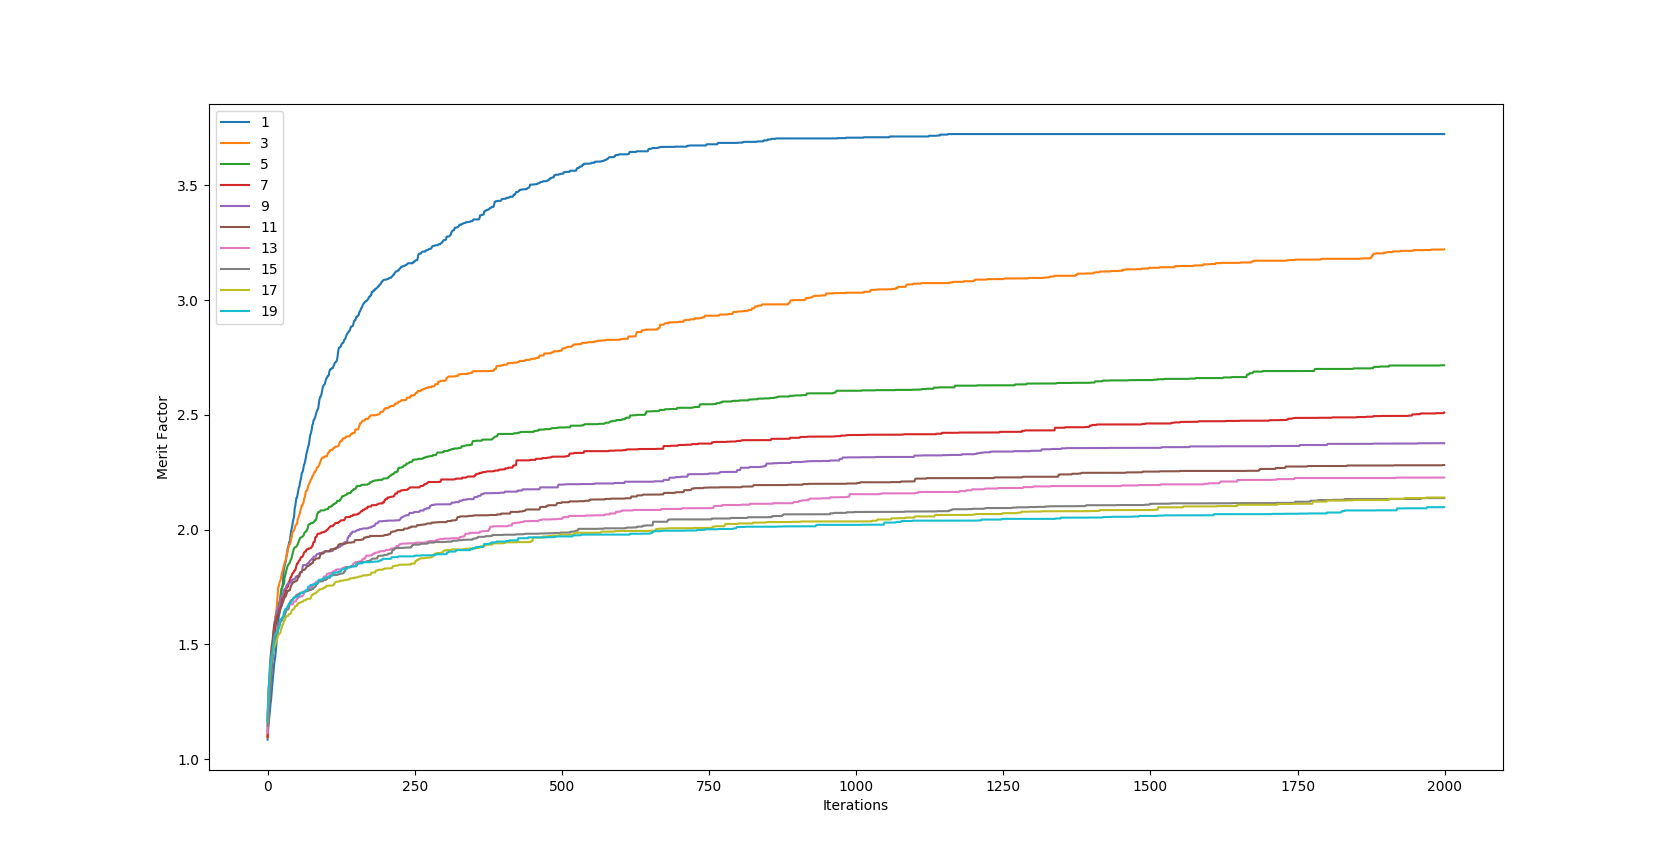
\includegraphics[scale=0.22]{Images/rls_nb_flip}
  \caption{Evolution of the merit factor with differents numbers of flips per iteration for the RLS algorithm.}
  \label{fig:rls_nb_flip}
  \end{center}
\end{minipage}%
\hfill
\begin{minipage}{.45\textwidth}
  \begin{center}
  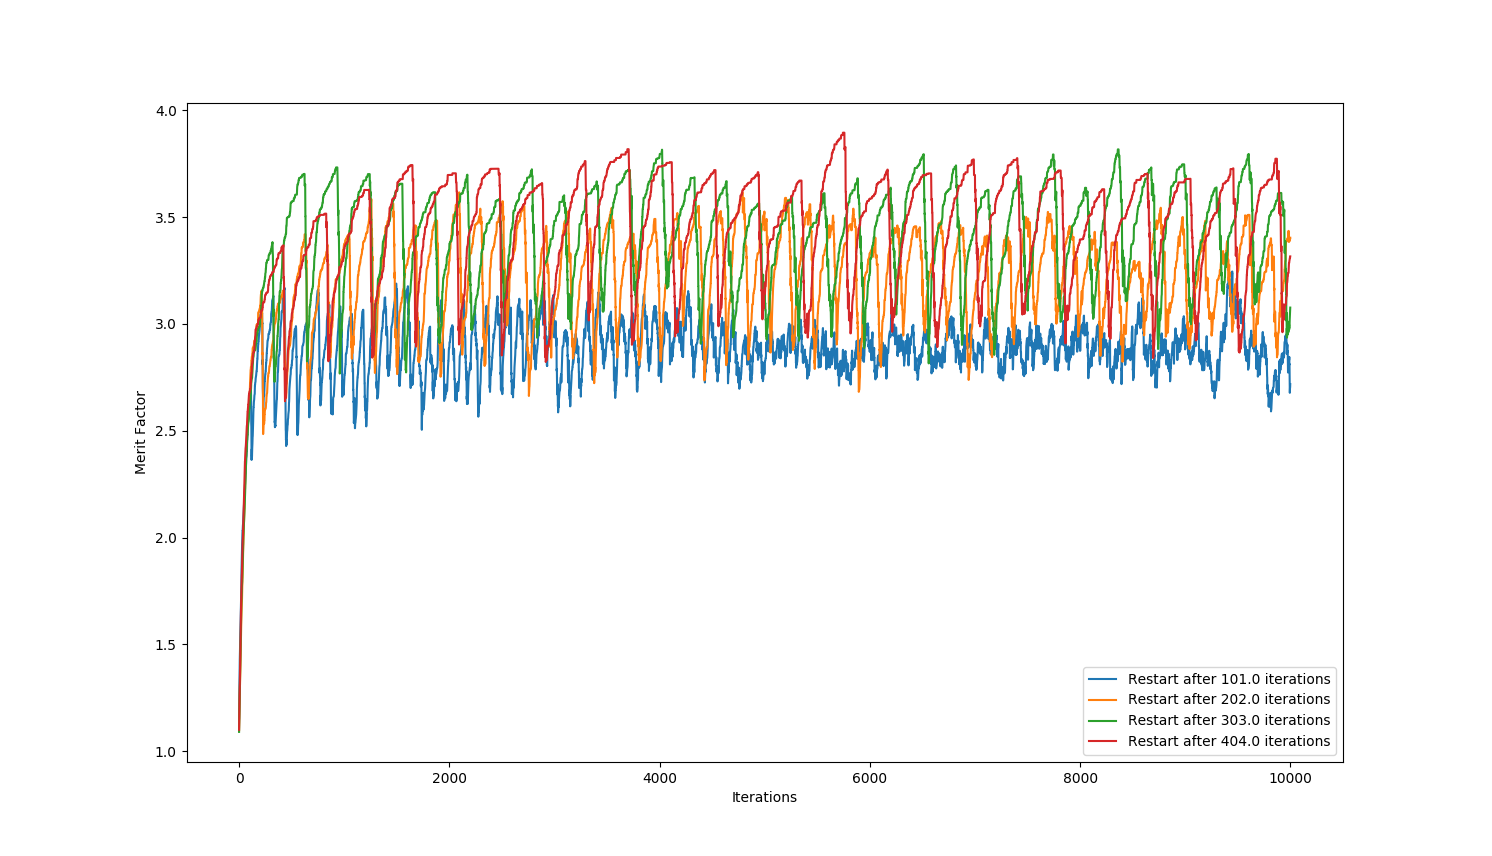
\includegraphics[scale=0.25]{Images/rls_no_change}
  \caption{Evolution of the merit factor with the RLS restart algorithm with $k=1$ and $k'=2$. We vary the number of iterations of no improvement (to the merit factor solution) before applying restart.}
  \label{fig:rls_no_change}
  \end{center}
\end{minipage}
\end{figure}
\begin{figure}[H]
\begin{center}
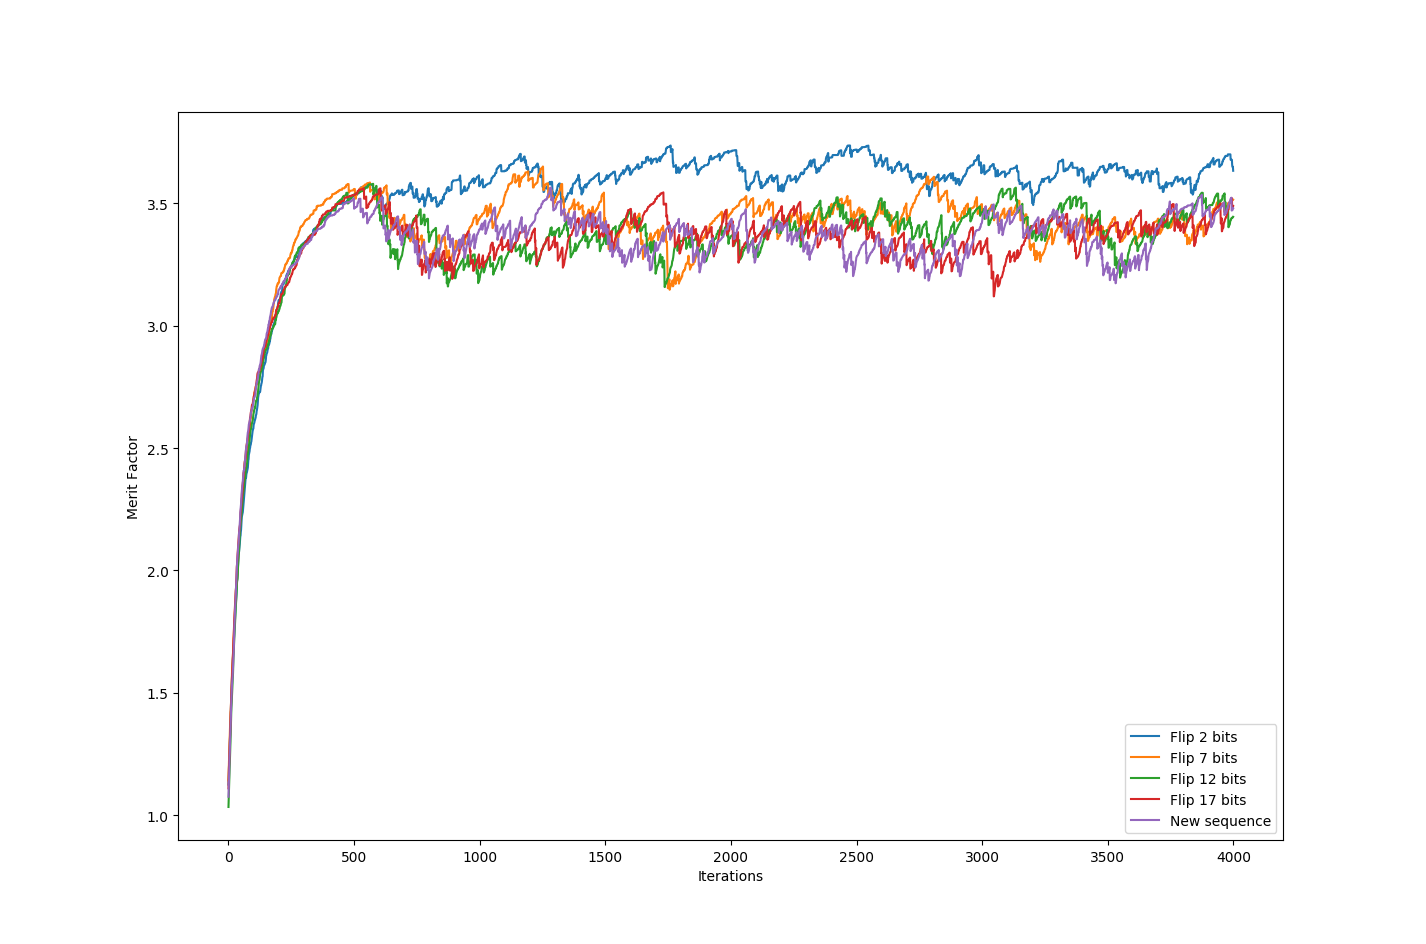
\includegraphics[scale=0.25]{Images/rls_restart}
\caption{Evolution of the merit factor algorithm with the RLS restart algorithm with $k=1$. We apply restart when the merit factor have not been improved for 3N iterations. We test 5 restart method : flipping 2,7,12 or 17 or a whole new sequence}
\label{fig:rls_restart}
\end{center}
\end{figure}
\noindent
We notice on fig \ref{fig:rls_nb_flip} that RLS algorithm stops making progress after some iterations because of this local maxima issue. Moreover, it seems that flipping more than 1 bit isn't effective.\\
To overcome the local minima issue of the RLS algorithm, we can do some transformations to the solution as soon as we do not improve our current solution for a fixed number of iterations. We call this new algorithm : RLS restart. There are two kind of transformations that can be easily implemented : start with a new sequence or flip $k'$ bits of the current solution. We can easily see on fig \ref{fig:rls_restart} that restart by flipping 2 bits (instead of 1) gives the best results. It's probably because we don't modify too much the solution found so far. On the other hand, flipping more than 2 bits or generating a whole new sequence are less effective. Moreover, we observe on fig \ref{fig:rls_no_change} that restarting too often isn't effective, it looks like restarting after 4N iterations gives the best results.
\section{EA (Evolutionary algorithm)}
\subsection{Definition}
\noindent
EA algorithm \cite{ea} is very close to the RLS one. However, rather than flipping a fixed number of bits per iteration, EA algorithm flips each bit independantly with a probability p.
\begin{enumerate}
\item Start with a random sequence which is your current solution
\item Pick a random neighbour of the current solution by flipping each bit of the current solution with a probability p
\begin{enumerate}
\item If this neighbour has a better merit factor than the current solution, use this neighbour as your current solution
\end{enumerate}
\item Go back to step 2 until the maximum number of iterations is exceeded
\end{enumerate}
\subsection{Tests}
\begin{figure}[H]
\begin{center}
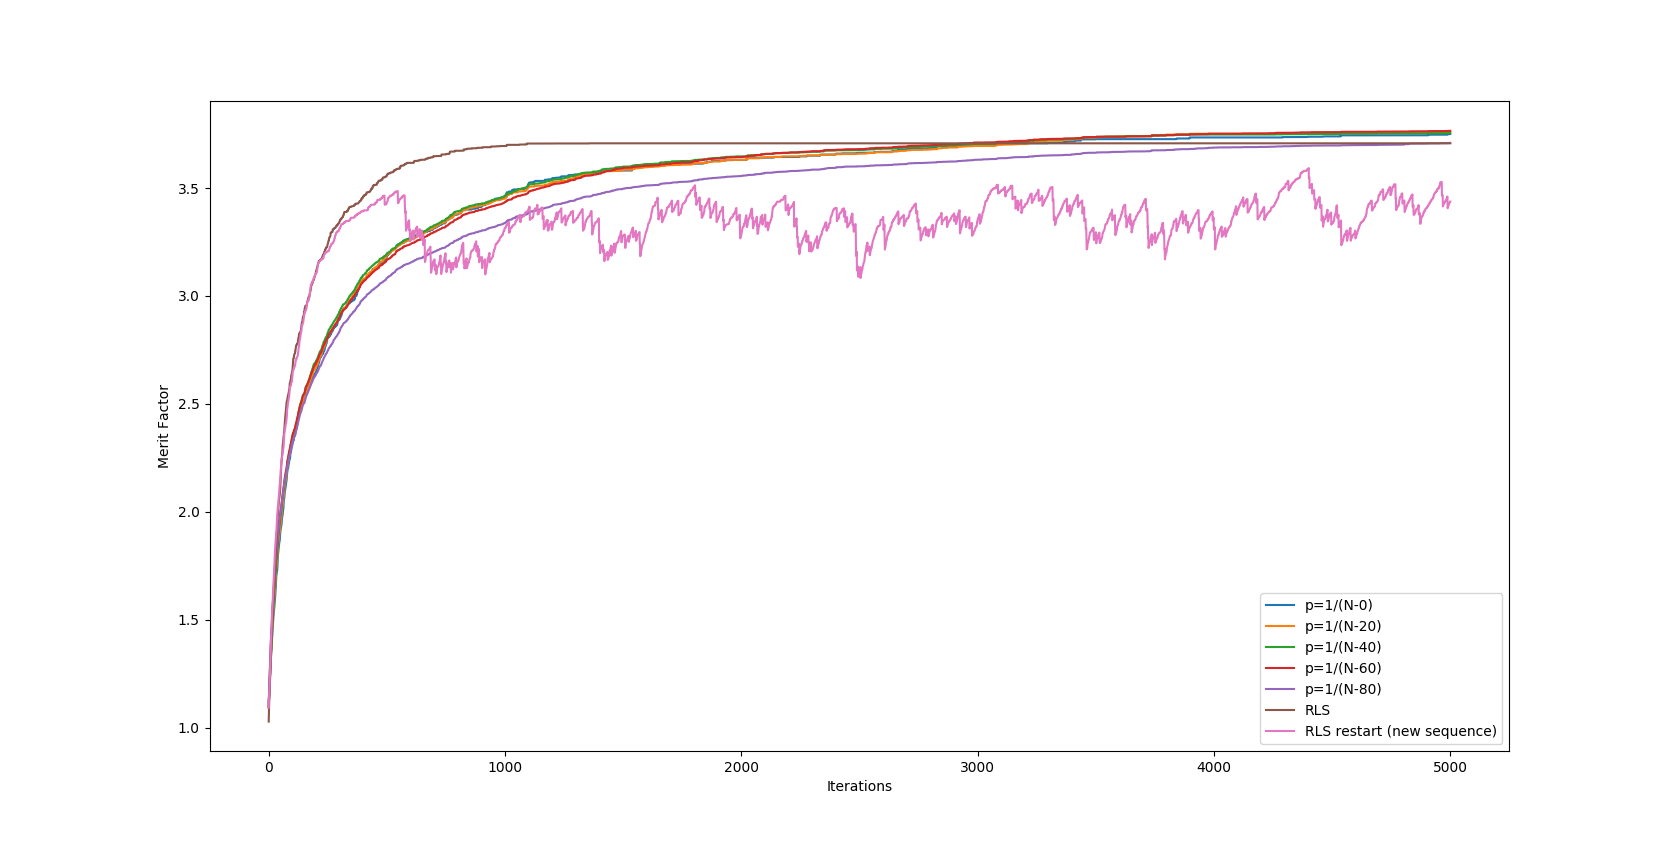
\includegraphics[scale=0.28]{Images/ea_different_p}
\caption{Evolution of the merit factor with RLS algorithm and EA algorithm with differents p}
\label{fig:ea_different_p}
\end{center}
\end{figure}
\noindent
We notice (fig \ref{fig:ea_different_p}) that EA algorithm with $p=\frac{1}{N}$ performs slightly better than the RLS algorithm while it should have the same behaviour on average. With this algorithm, we take avantage of the random behaviour of the bit flipping. Indeed, in average, the algorithm should flip only 1 bit, but this is only an average behaviour and doesn't prevent the algorithm to sometimes flip more than one bit and escape from a local maxima. Regarding the other values of $p$, we can't say anything because the gap between each other isn't significant.
\section{Simulated Anealing}
\subsection{Definition}
\noindent
For the RLS and EA algorithm, we were only accepting solutions which had a better merit factor than the current solution. Here \cite{sa}, we accept any neighbour which has a better merit factor but we also sometimes accept solutions which don't improve our current solution. However the probability $p$ that we accept a poorer solution evolves over time and also depends on the change of the merit factor.
\begin{equation}
p=e^{(f_y-f_x)\cdot t}
\end{equation}
$f_x=$ Merit factor of the current solution $x$\\
$f_y=$ Merit factor of a neighbour $y$ of our current solution $x$ ($f_x>f_y$)\\
So, there are two factors which decrease the probability $p$ to take a neighbour $y$ which has a poorer merit factor :
\begin{itemize}
\item Its merit factor $f_y$ is way worse than our current merit factor $f_x$
\item $t$ is big (meaning we have already done many iterations)
\end{itemize} 
From now on, we need to choose how t increases over time, mainly 3 solutions are possible :
\begin{itemize}
\item Linearly
\item Exponentially
\item Logarithmically
\end{itemize}
Additionally to the kind of growth of $t$, we need to choose $t_{max}$, which is the value of $t$ at the end of the algorithm (assuming we have a fixed number of iterations). This parameter is critical because a low value means often accepting poorer solutions and a high value means never  to accept poorer solutions (i.e equivalent to RLS). We could have choosen not to bound $t$ but it would have been complicated to compare different kinds of growth because the value at the end would have been completely different. So here is the algorithm :
\begin{enumerate}
\item Start with a random sequence which is your current solution $x$, compute its merit factor $f_x$
\item Pick a neighbour $y$ of the current solution $x$ by flipping each bit of the current solution with a probability p
\item Compute the merit factor $f_y$ of $y$
\begin{enumerate}
\item If $f_y\geq f_x$, then $x:=y$ and $f_x:=f_y$
\item If $f_y<f_x$ and random\_number\footnote{The random number must be in [0,1]}$<$p then $x:=y$ and $f_x:=f_y$
\end{enumerate}
\item Go back to step 2 until the number max of iterations is exceeded
\end{enumerate}
\subsection{Tests}
\begin{figure}[H]
\centering
\begin{minipage}{.45\textwidth}
  \begin{center}
  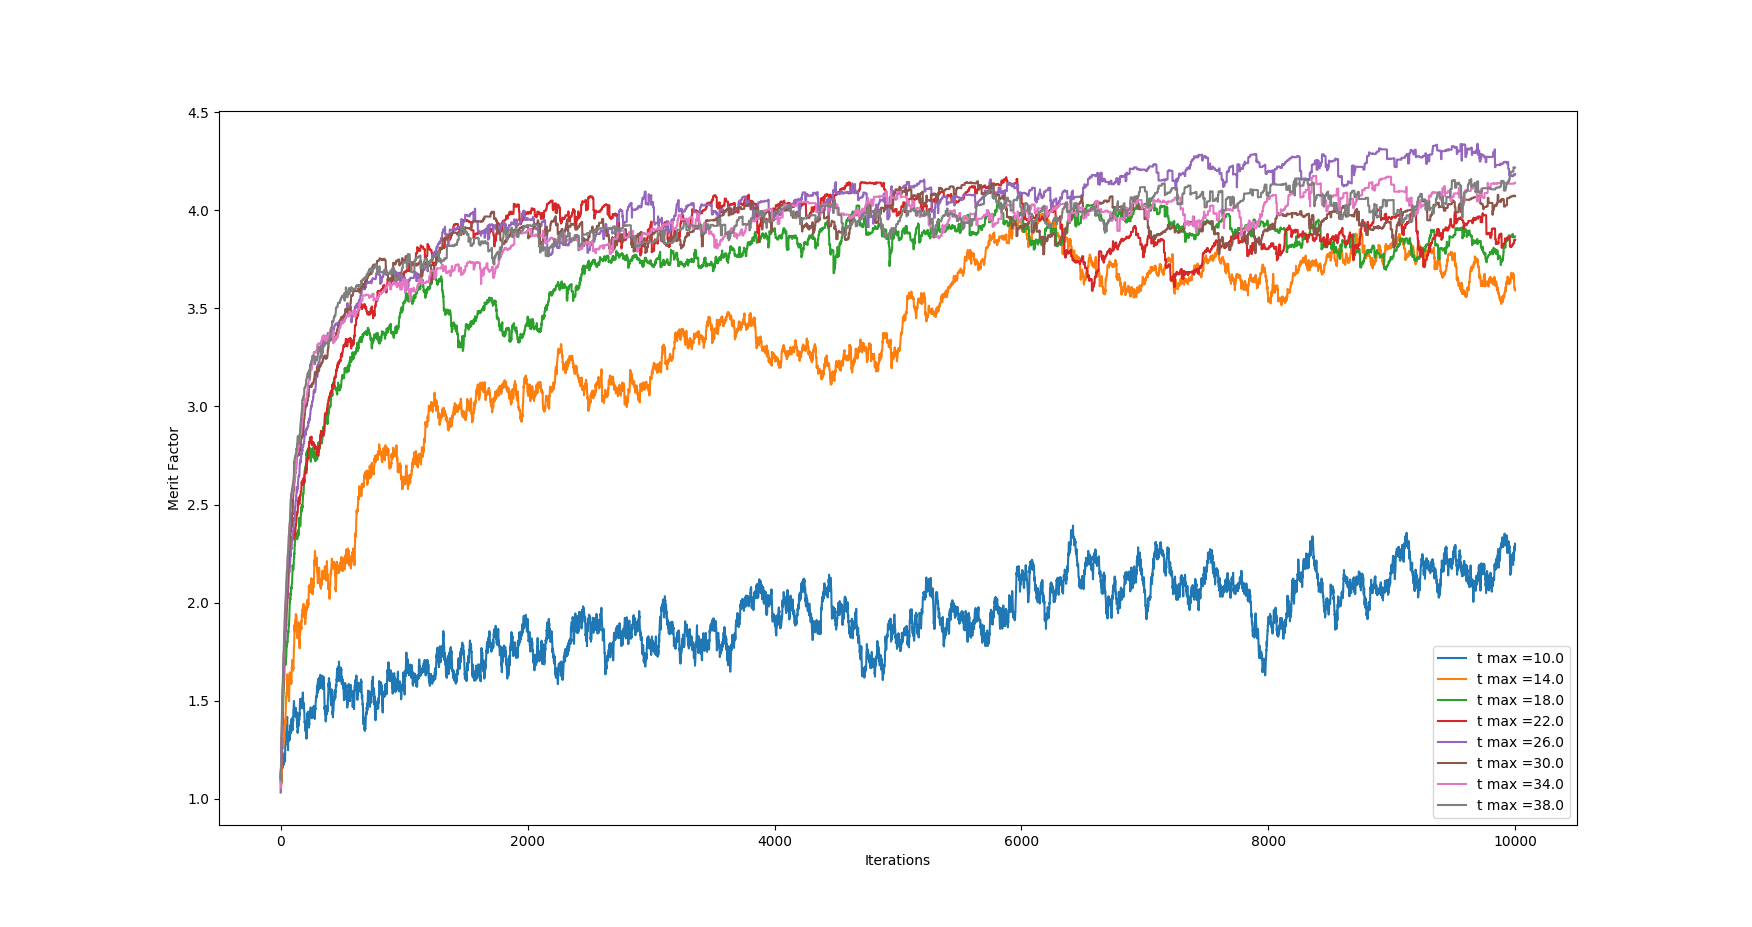
\includegraphics[scale=0.23]{Images/sa_tmax}
  \caption{Evolution of the merit factor with the simulated anealing algorithm with different values for $t_{max}$. The growth of $t$ is linear and we select neighbour by flipping randomly one bit.}
  \label{fig:sa_tmax}
  \end{center}
\end{minipage}%
\hfill
\begin{minipage}{.45\textwidth}
  \begin{center}
  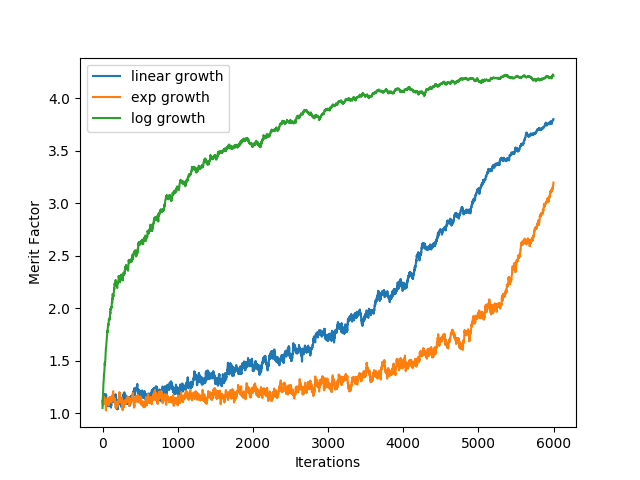
\includegraphics[scale=0.4]{Images/sa_growth}
  \caption{Evolution of the merit factor with the simulated anealing algorithm with respect to the kind of growth for $t$ while $t_{max}=15$.}
  \label{fig:sa_growth}
  \end{center}
\end{minipage}
\end{figure}
\noindent
Fixing a low $t_{max}$ (i.e $\leq 13$) isn't productive and induces a slow growth (fig \ref{fig:sa_tmax}). Instead, choosing the value of $t_{max}$ around 18 seems to be the right choice. Regarding the growth of $t$, a logarithmic growth quickly gives a good solution whereas the linear and exponential growths are way slower.
\section{Monte Carlo Search}
\subsection{Definition}
\noindent
A Monte Carlo tree search \cite{mc} is a heuristic which is often used in artifical intelligence in games such as Chess or Go. The aim of the heuristic is to find the next most promising move given a game state. A tree is created at the beginning. Then we need to choose the node of the tree which is the most promising and add randomly leaves to this node (which are actually neighbours of this node).\\
In our case, each node is a sequence, and we evaluate each node with its merit factor. The algorithm is :
\begin{enumerate}
\item Generate a sequence randomly and set it as the root of the tree
\item Choose the most encouraging node of the tree based either on :
\begin{enumerate}
\item Its merit factor
\item Its "merit factor back"
\item Its UCT
\end{enumerate}
\item Add a fixed number of neighbours as leaves to this node and compute their merit factor
\item Update the "merit factor back" of all their ancestors
\item Go back to step 2 until a good solution is found
\end{enumerate}
The UCT of a node is :
\begin{equation}
UCT=\frac{merit\;factor\;back}{n}+c\sqrt{\frac{ln(N)}{n}}
\end{equation}
$n=$ Number of time the node has been visited\\
$N=$ Number of time the father of this node has been visited\\
$c=$ Exploration parameter (most of time equal to $\sqrt{2}$)\\\\
The "merit factor back" of a node is a value which takes into account its own merit factor and those of all its descendants\footnote{In the original Monte Carlo algorithm, once a node has been visited, we update the value of all its ancestors.}. So, each time we compute the merit factor of a node, we need to compute the "merit factor back" of all its ancestors (fig \ref{fig:mc_tree}). The way we update its ancestors will be discussed in the next part. In this fashion, looking at the "merit factor back" of a node is like checking if this node has good descendants. 
\subsection{Tests}
\begin{figure}[H]
\centering
\begin{minipage}{.45\textwidth}
  \begin{center}
  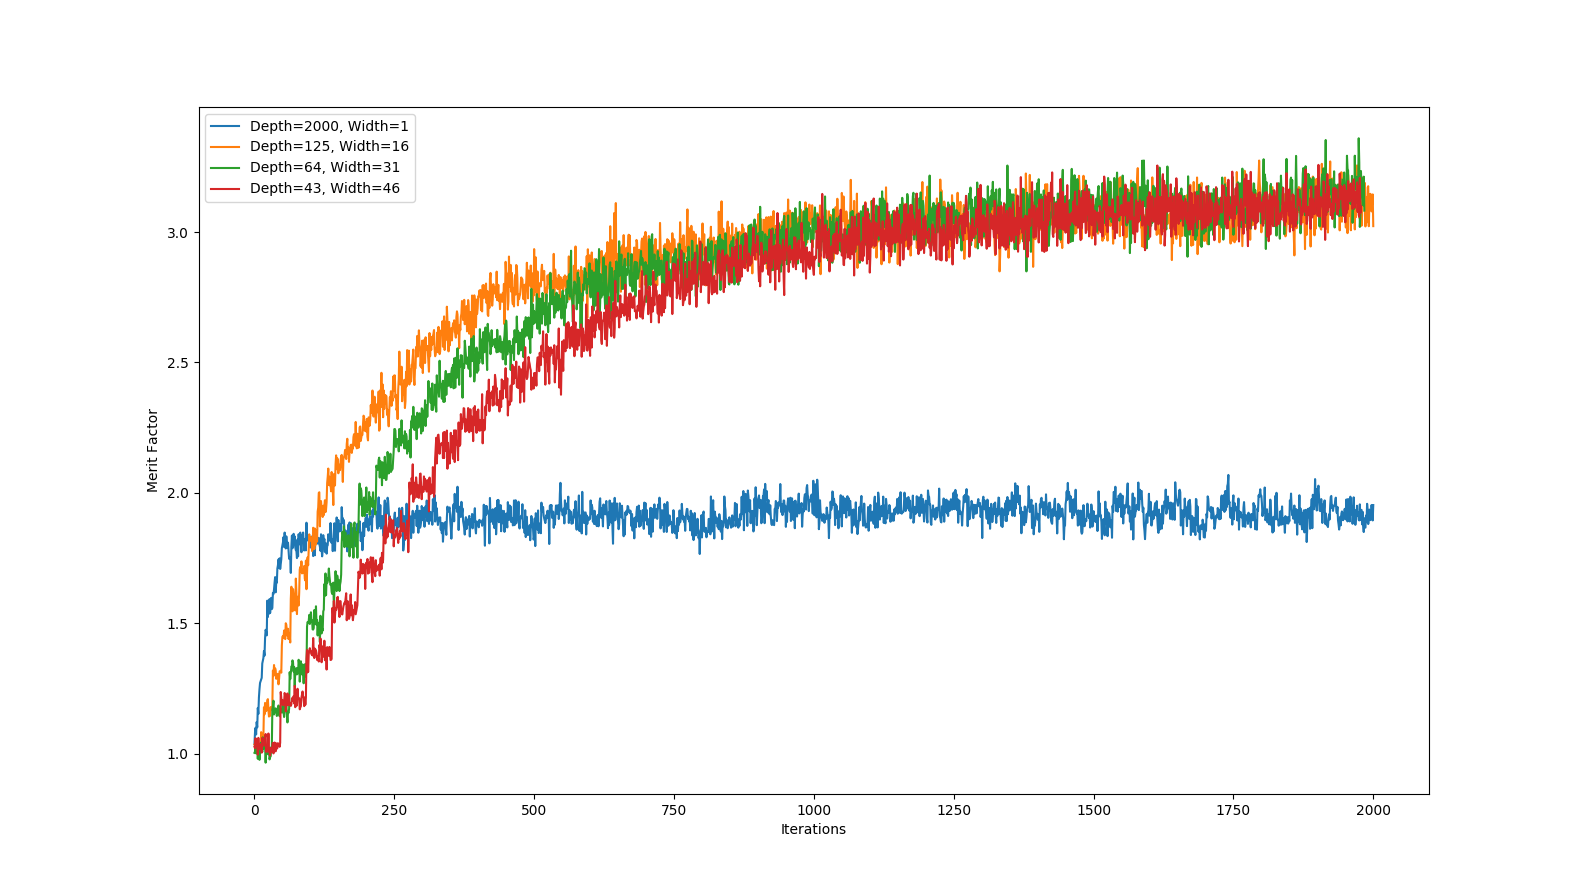
\includegraphics[scale=0.21]{Images/mc_width_depth}
  \caption{Evolution of the merit factor with the Monte Carlo algorithm with various values for the width and for the depth of the tree}
  \label{fig:mc_width_depth}
  \end{center}
\end{minipage}%
\hfill
\begin{minipage}{.45\textwidth}
  \begin{center}
  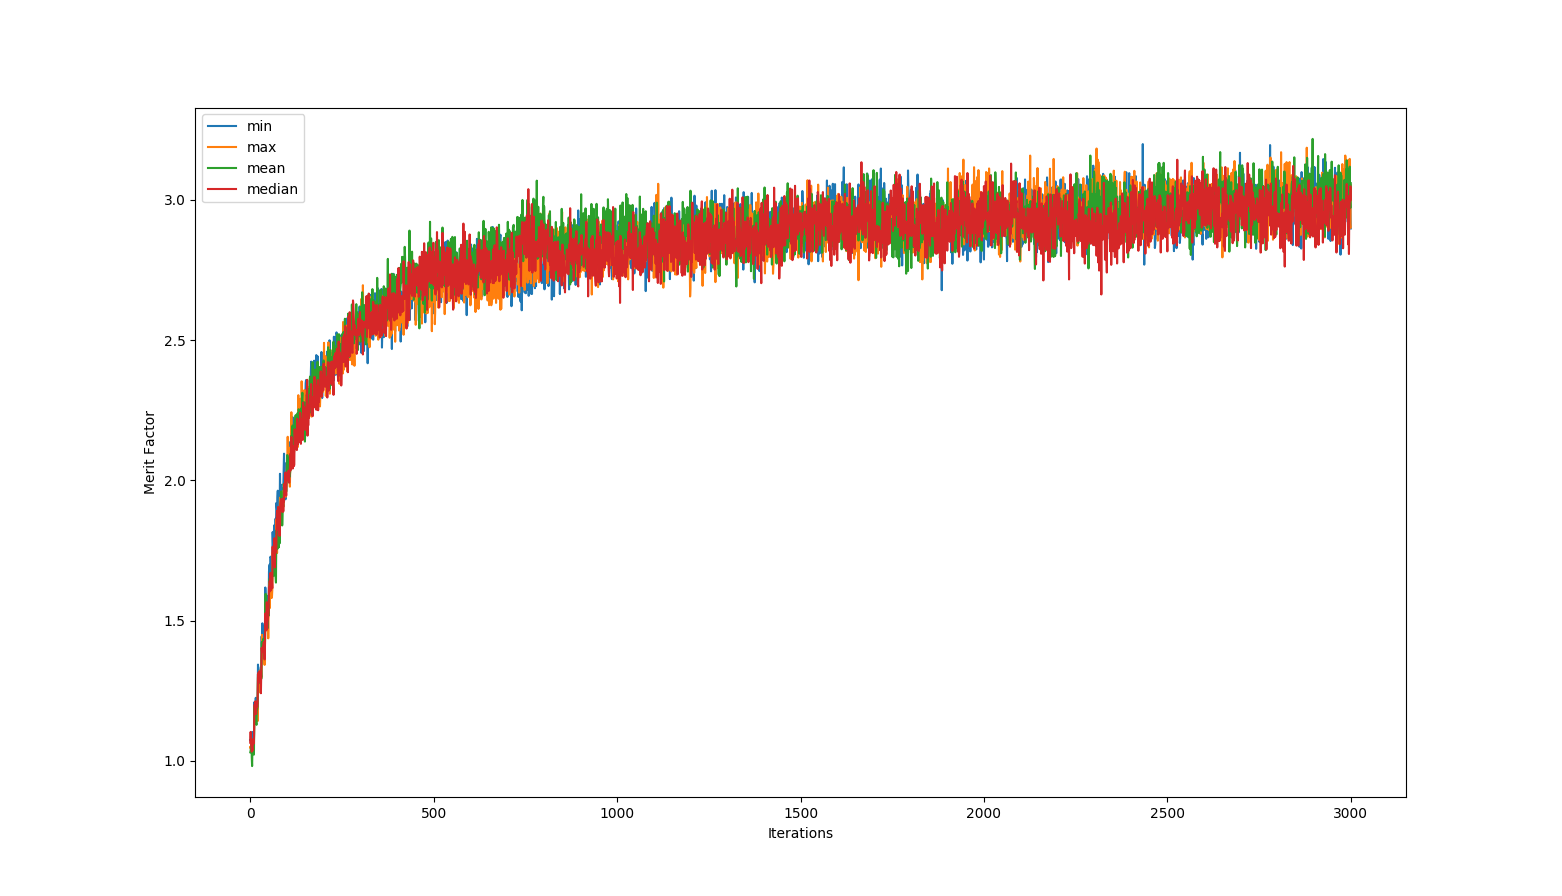
\includegraphics[scale=0.21]{Images/mc_merit_factor_back}
  \caption{Evolution of the merit factor with the Monte Carlo algorithm with different ways to choose the next parent}
  \label{fig:mc_merit_factor_back}
  \end{center}
\end{minipage}
\end{figure}
\noindent
In the fig \ref{fig:mc_width_depth} and fig \ref{fig:mc_merit_factor_back}, we are not actually looking at the number of iterations but rather the number of nodes. Indeed, in the previous algorithms, we were only looking at 1 neighbour at a time but in this case we add a fixed number of neighbours at each iteration. So reasoning only about the number of iterations is biaised because we are actually looking at way more solutions.\\
Furthemore, it seems that the number of neighbours we add at each iteration is not a decisive argument. We notice on fig \ref{fig:mc_width_depth}, that adding one neighbour at a time is a bad idea. From another angle, the way we update our ancestors (fig \ref{fig:mc_merit_factor_back}) doesn't seem to have any importance. We can update the merit factor of a parent by taking the mean/median/max/min of the merit factor of its children and its own without too much consideration. However the metric used to choose the next node to add children to is more important (fig \ref{fig:mc_choose_children}). As expected, choosing a node on its merit factor is similar to the RLS algorithm. Apart of that, choosing the UCT value or the "merit factor back" seems to induce the same behaviour.
\begin{figure}[H]
\begin{center}
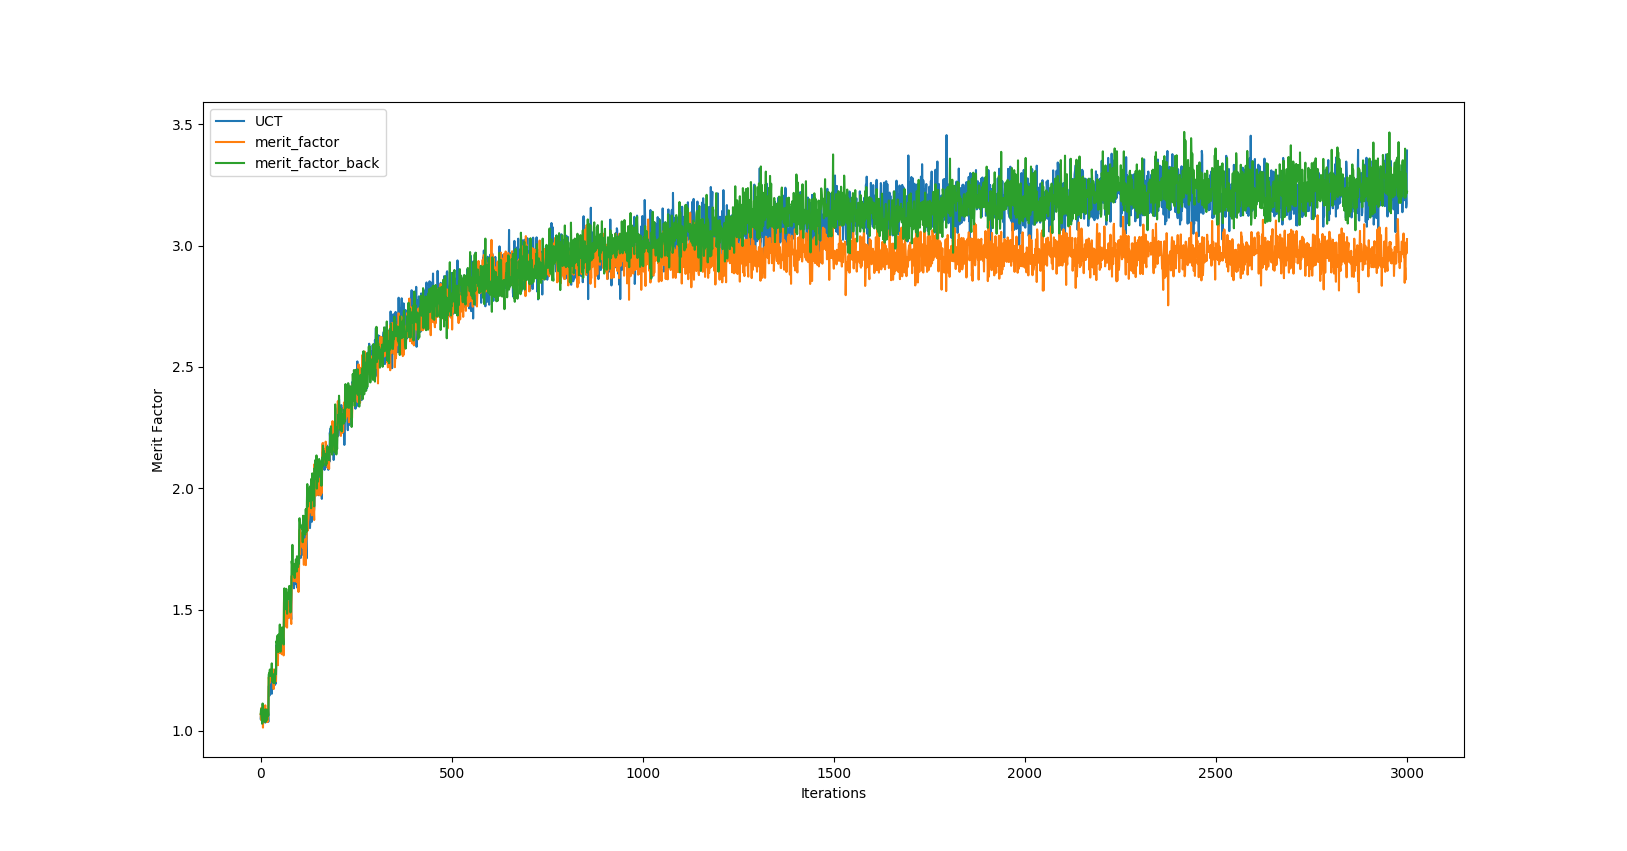
\includegraphics[scale=0.22]{Images/mc_choose_children}
\caption{Evolution of the merit factor with the Monte Carlo algorithm by varying the way to choose the node to add a children to (adding 20 neighbours at a time).}
\label{fig:mc_choose_children}
\end{center}
\end{figure}
\begin{figure}[H]
\begin{center}
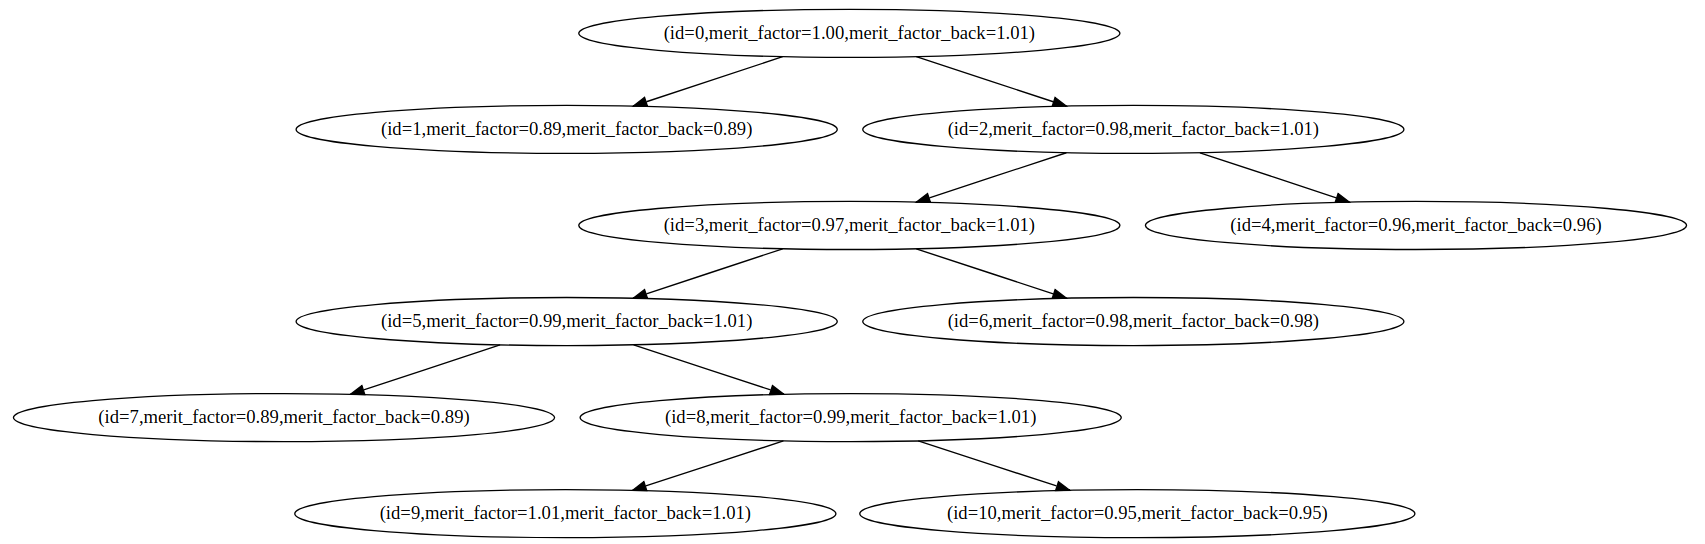
\includegraphics[scale=0.3]{Images/mc_tree}
\caption{Example of tree with the Monte Carlo algorithm. The "merit factor back" is computed using the max of the children. The node with id=9 has the biggest merit factor. All the "merit factor back" of its ancestors take its value.}
\label{fig:mc_tree}
\end{center}
\end{figure}
\section{Analysis}
\subsection{Merit Factor}
\begin{figure}[H]
\begin{center}
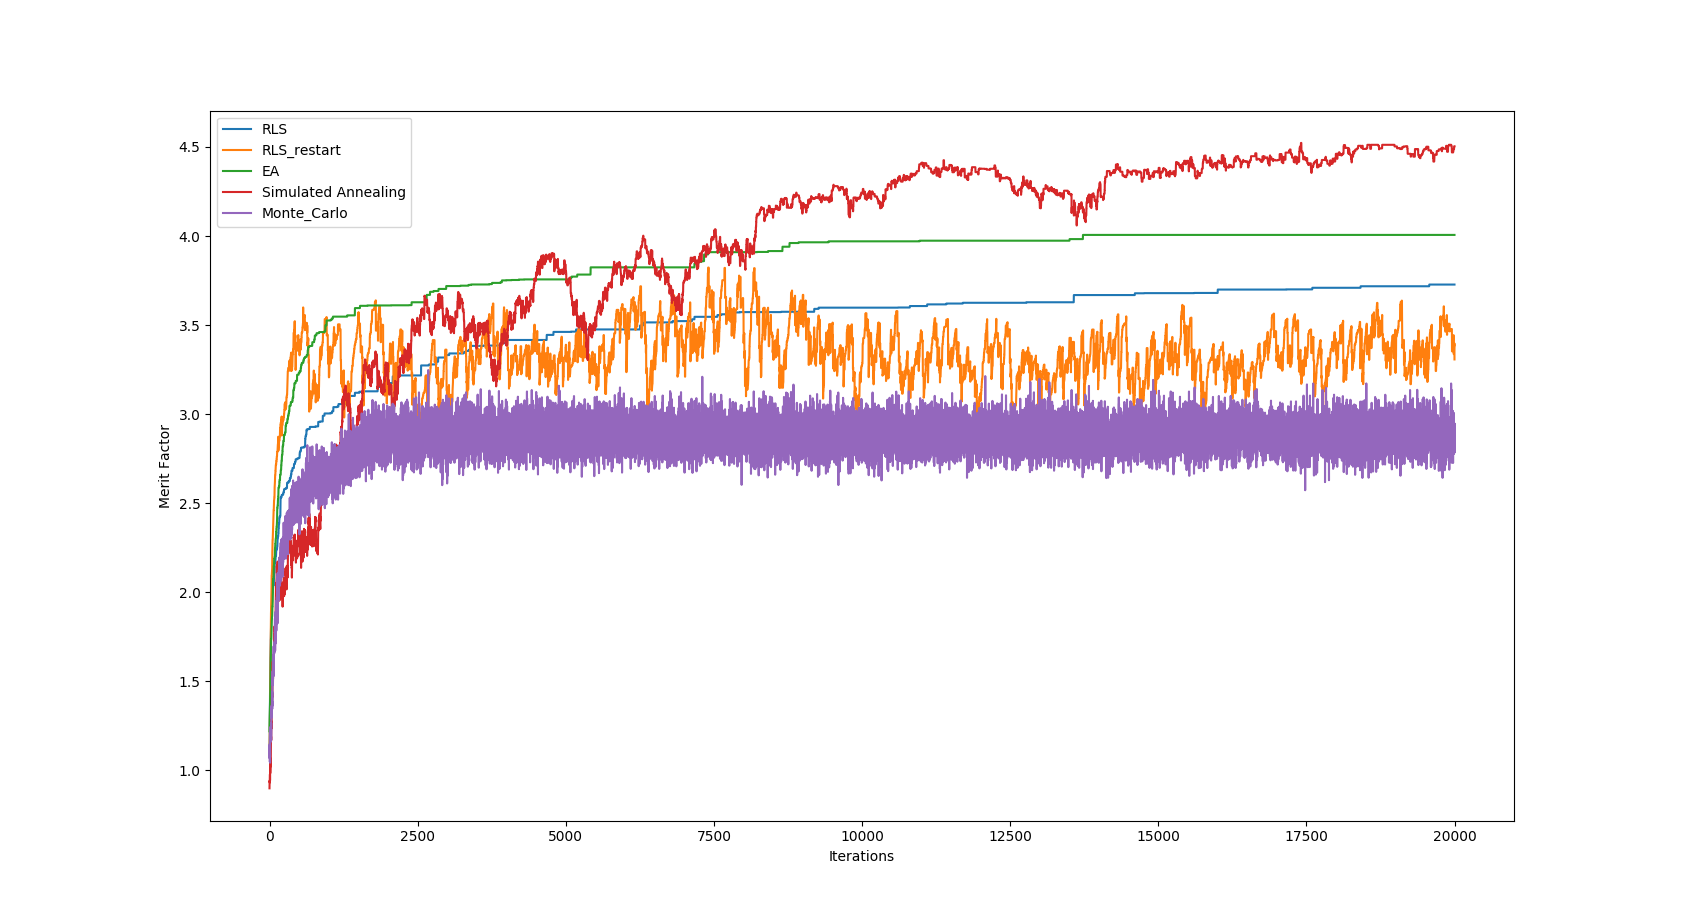
\includegraphics[scale=0.35]{Images/all_results}
\caption{Evolution of the merit factor with the following heuristics : RLS (number of flip=1), RLS with restart (number of flip=1,restart with 2 flips), EA(p=$\frac{1}{N}$), Simulated Anealing (number of flip=1, $t_{max}=20$, growth=log), Monte Carlo Search (width=20)}
\label{fig:all_results}
\end{center}
\end{figure}
\noindent
We have gathered all the algorithms presented before with the best parameters found so far. The best algorithm seems to be the simulated anealing (fig \ref{fig:all_results}). However, this is only a mean over 50 runs, and it doesn't show the best value computed by each algorithm.\\
\begin{center}
\begin{tabular}{|c|c|c|c|c|c|}
\hline
  & RLS & RLS restart & EA & Simulated Anealing & Monte Carlo \\
\hline
Best Merit Factor & 4.48 & 4.34 & 4.67 & 5.11 & 5.32\\
\hline
\end{tabular}
\end{center}
Although the growth of the Monte Carlo algorithm seems slow compared to the other, it's actually the algorithm which finds the best solution.

\subsection{Size of the instance}
Since the begining of this report, we have only been testing sequences of length 101. It would be interesting to see if the length of the sequence is actually important in the performance of an algorithm.
\begin{figure}[H]
\begin{center}
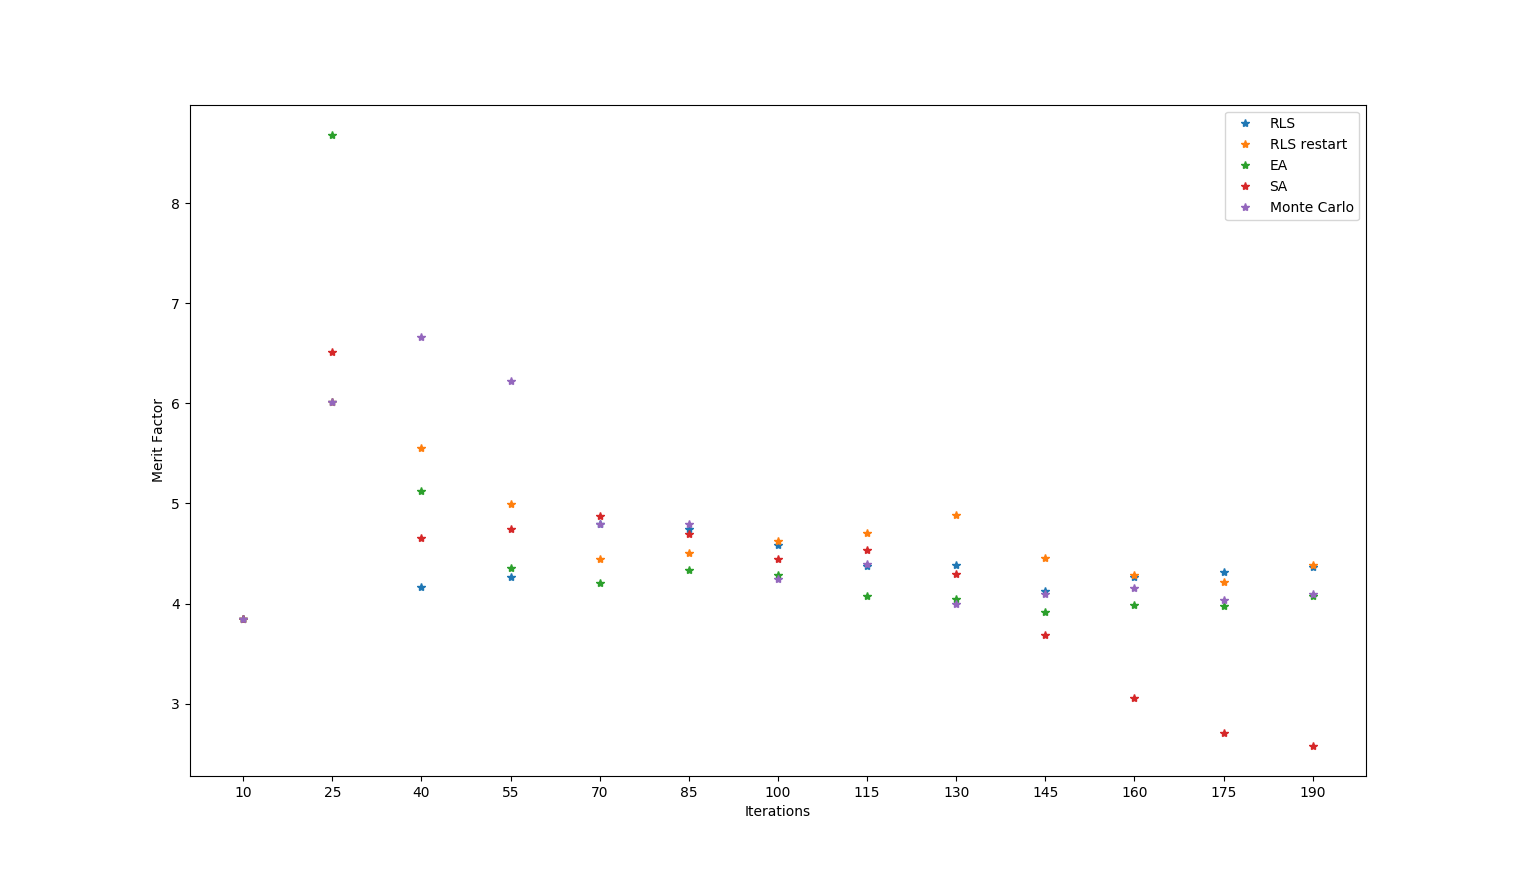
\includegraphics[scale=0.26]{Images/instance_size}
\caption{Best merit factor found by all the algorithms by varying the size of the instance (i.e sequence).}
\label{fig:instance_size}
\end{center}
\end{figure}
\noindent
The instance size seems to actually matter. The simulated anealing algorithm works quite well on small instances ($\leq 120$) but not so good on bigger instances. From another angle, the RLS with restart algorithm seems on average not bad at all. Our choice to evaluate the algorithms on instances of size 101 is finally a good choice because (based on fig \ref{fig:instance_size}) it reflects an average behaviour.
\subsection{CPU usage}
The memory usage is almost non-existent because we are using only 3 variables in the first four algorithms. In the Monte Carlo algorithm, the memory usage is a bit higher because we save the merit factor and the sequence for each node visited (but very low).\\
Regarding the time spent by each algorithm, the first four algorithm spend almost the same time (0.5 seconds for 1000 iterations) but the Monte Carlo algorithm lasts 7 times more time than the others.
\begin{figure}[H]
\begin{center}
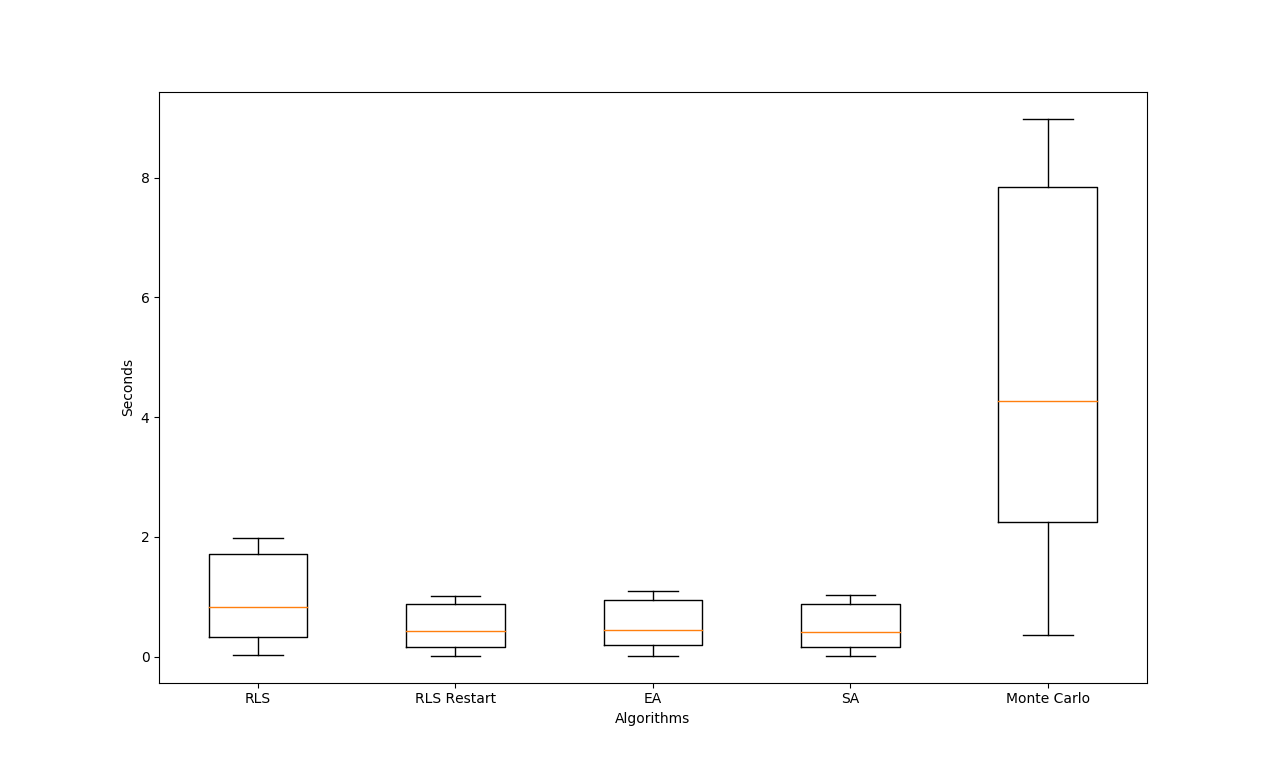
\includegraphics[scale=0.26]{Images/time_spent}
\caption{Time spent by each algorithm for 1000 iterations on average over 100 runs with instances with size from 10 to 200.}
\label{fig:time_spent}
\end{center}
\end{figure}
\subsection{Make the sequence stationnary}
\noindent
The LABS problem tries to maximize the merit factor $M(S)$ of a sequence $S$. However this metric is too sensitive to change, meaning that if you change only one bit of the sequence, the result may be completely different. This is a big issue because it makes the learning way more difficult.\\
So the idea is to find another way (less volatile) to evaluate the quality of a solution. By looking at the best results into the github file (\url{https://github.com/borkob/git_labs/blob/master/results-2018/2016-labs-skew.txt}), we notice something quite surprising : all the sequences have something in common : the number of changes. It's not easy to see it with this natural form. Howewer, it's obvious once you get your sequence stationary. A stationary sequence is a sequence whose probability distribution is invariant over time (to avoid seasonality for instance). A simple way to get a sequence $S=(s_1,...,s_N)$ to its stationary form is to do : $s_i=s_{i+k}-s_i$ where $k\in [1,N-k]$.\\
And surprisingly, absolutely all the solutions of the file verify this equation :
\begin{equation}
\sum_{i=1}^{N-k} |s_{i+k}-s_{i}|=N-k \;\, \forall k \; odd\; \in [1,N-1]
\end{equation}
So, for a sequence S of length N, it creates a system of $\ceil{\frac{N-1}{2}}$ equations. For instance, when N=5 we have 2 equations :
\begin{equation}
\begin{split}
|s_2-s_1|+|s_3-s_2|+|s_4-s_3|+|s_5-s_4|&=5-1=4\\
%|s_3-s_1|+|s_4-s_2|+|s_5-s_3|&=5-3=2\\
|s_4-s_1|+|s_5-s_2|&=5-3=2\\
%|s_5-s_1|&=\ceil{\frac{5-4}{2}}=1\\
\end{split}
\end{equation}
You can check that with this sequence (the one in the github file) : [-1,-1,-1,1,-1], it works.\\
Thus, it might be better to optimize the mean absolute error of this sytem [\ref{eq:MAE}], meaning summing the absolute value of the error for each equation.
\begin{equation}
\label{eq:MAE}
MAE(S)=\frac{1}{N-1}\sum_{k=1 \text{ and k odd}}^{N-1}|\sum_{i=1}^{N-k} |s_{i+k}-s_{i}|-(N-k)|
\end{equation}
We can't solve this system using a linear system solver nor by using the simplex algorithm because the system isn't linear (contains absolute values). So the heuristic seems to be the right choice.
Furthemore, we want to minimize this error, so we can apply the heuristics explained before by multiplying the result by -1 (to transform minimization into maximization).\\
\subsubsection{Why optimizing this new function ?}
\noindent
However, let's take a step back. The reason we needed a new heuristic was to get a smooth heuristic which, ideally wouldn't be too volatile. So we need to check wether or not it's the case.\\
In order to test it, we generated 10000 sequences of length 101. For each of these sequences, we flip one bit randomly and comparate the value of the MAE before and after flipping one bit.\\
\begin{figure}[H]
\begin{center}
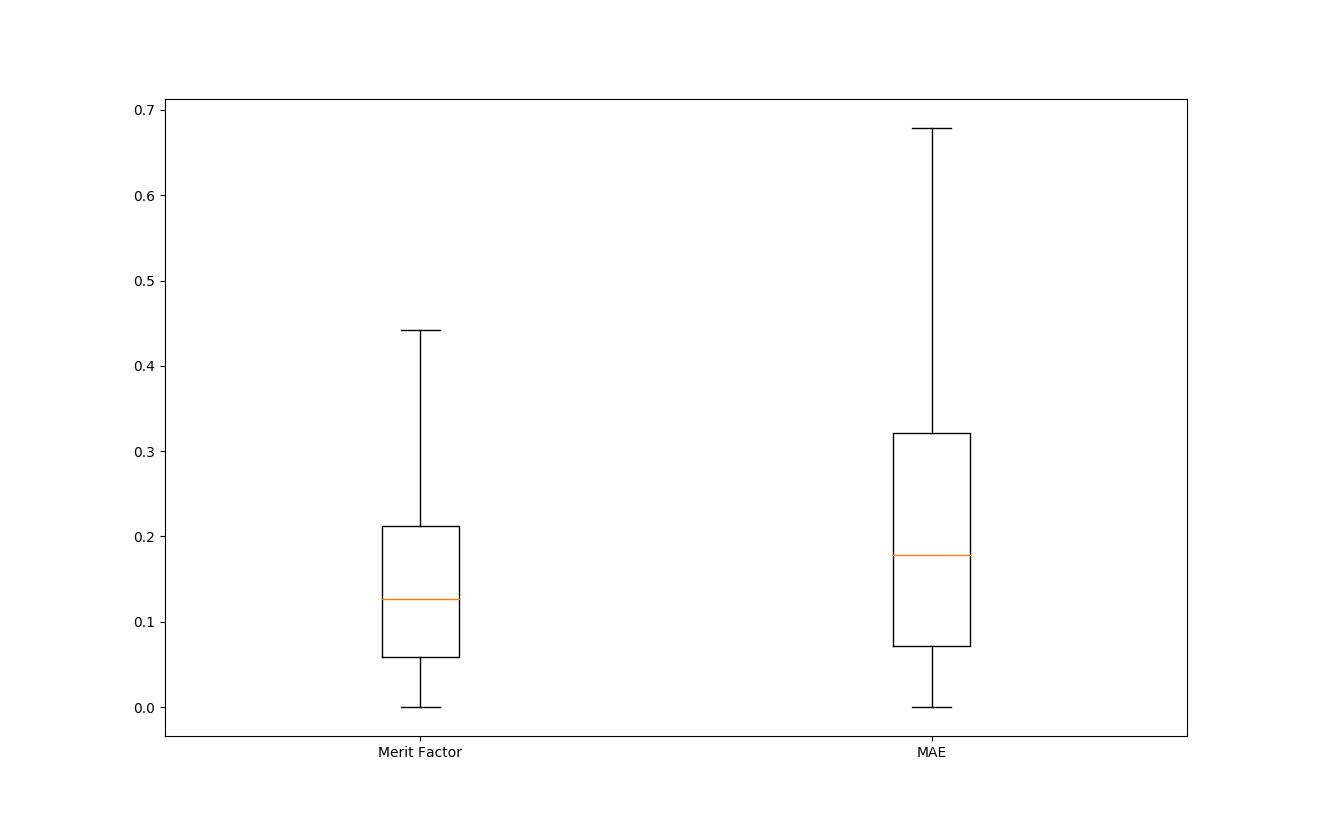
\includegraphics[scale=0.2]{Images/compare_mf_mae}
\caption{Comparison of the gap for a sequence before and after flipping one bit. Both metrics have been normalized ($\bar{x}=\frac{x-min}{max-min}$)}.
\label{fig:compare_mf_mae}
\end{center}
\end{figure}
\noindent
On fig \ref{fig:compare_mf_mae}, we notice that flipping one bit changes even more the MAE function. Thus, our new heuristic is even worse than the merit factor function. The only benefit of this function is that in average over 10000 runs, it takes twice less time to compute it than the merit factor. Although this new function doesn't seem to be a good choice, let's see how it performs.
\begin{figure}[H]
\begin{center}
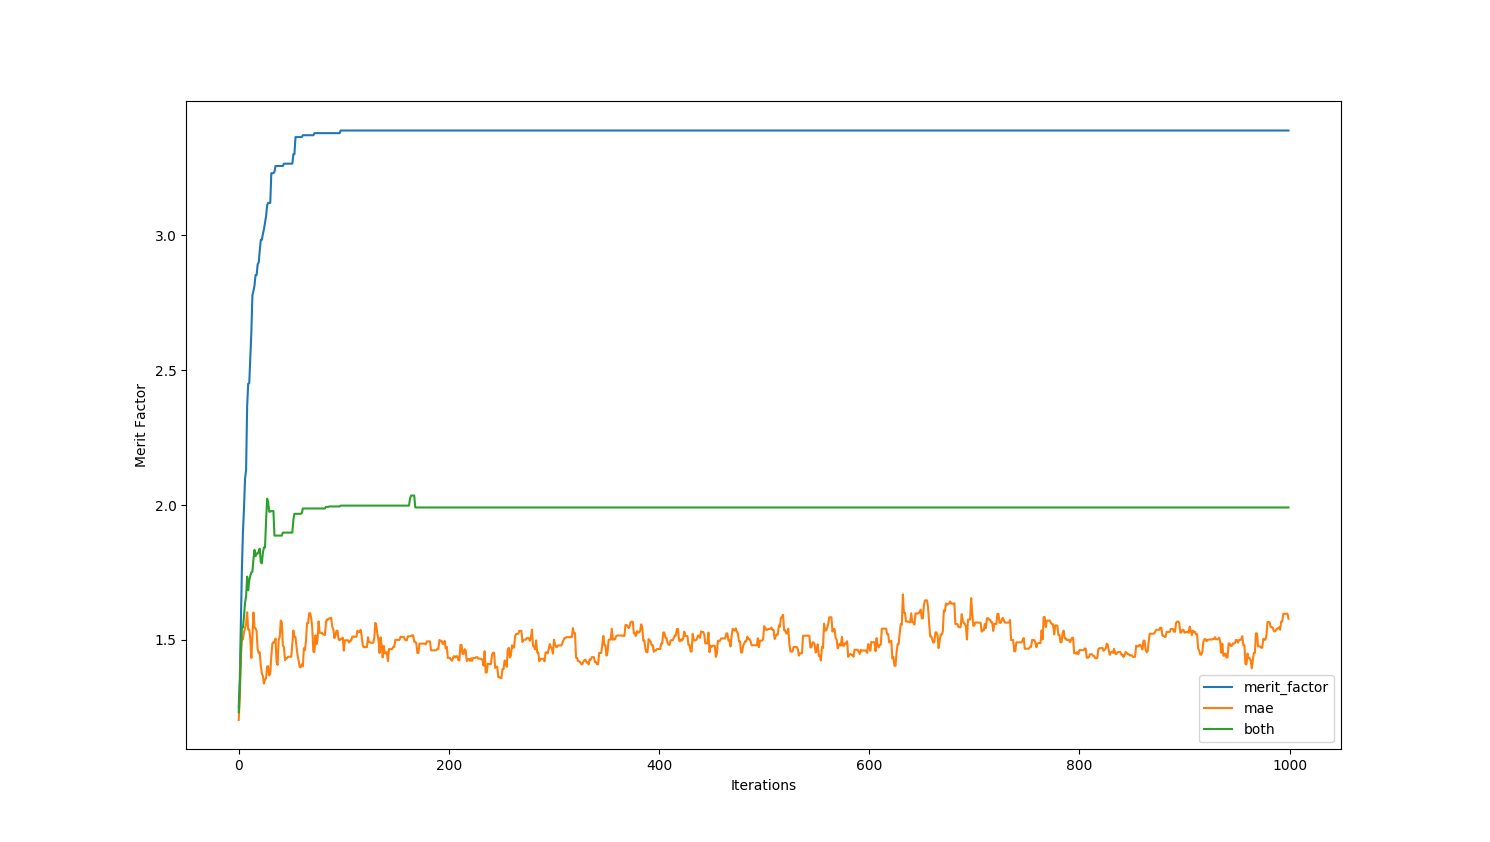
\includegraphics[scale=0.22]{Images/rls_both_heuristics}
\caption{Evolution of the merit factor with RLS when optimizing the merit factor, the MAE just mentioned before and the mean of both.}
\label{fig:rls_both_heuristics}
\end{center}
\end{figure}
\noindent
Unfortunetely, it seems on fig \ref{fig:rls_both_heuristics} that optimizing this new heuristic doesn't work at all. It may be explained by the lack of information. Indeed, we have $N$ unknown values but we only compute the mean over $\ceil{\frac{N-1}{2}}$ equations.\\

\subsection{Quantum application}
\DeclarePairedDelimiter\bra{\langle}{\rvert}
\DeclarePairedDelimiter\ket{\lvert}{\rangle}
\noindent
Quantum algorithm can sometimes offer a great speedup compared to classical algorithms. In particular, the use of Grover's algorithm \cite{search} and period finding algorithm are at the core of many quantum algorithms. In our case, the use of Grover's algorithm is well suited. Grover's algorithm enables to look for an element in a set of $N$ elements in $O(\sqrt{N})$ instead of $N$ (which is a quadratic speedup).
Suppose we have an oracle $f$ :\\\\
$f_i(j)=\left\{
\begin{array}{l}
  1 \text{ if MF[$j$] $>$ MF[$i$]} \\
  0 \text{ otherwise}
\end{array}
\right.$\\\\
where MF[i] is the merit factor of the sequence i\\\\
Here is the algorithm :
\begin{enumerate}
\item Let n be the length of the sequence and $N=2^n$ the number of states
\item Choose an index $y \in \{0,..,N-1\}$
\item Begin with the state $\ket{\phi}=\ket{0}\ket{y}$
\item Get the state $\ket{\phi}=\frac{1}{\sqrt{N}}\sum_{i=0}^{N-1}\ket{i}\ket{y}$ by applying Hadamard transform on the first register
\item Apply Grover's algorithm to get one marked state (i.e a state with $f_y(x)=1$)
\item Make a measurement on the first register. This value will be our new $y$
\item Go back to step 3 until $\sqrt{N}$ iterations have been done
\end{enumerate}
This algorithm is extracted from the paper \cite{max_quantum}. Hence we are able to find the sequence with the maximum merit factor in $\sqrt{N}$ steps. The only requirement is to get a system of $n$ qubits and the oracle $f$.
\section{Conclusion}
\noindent
This report is much longer than expected but some informations needed to be explained. To conclude, we can't say that any heuristic developped in this report performs well. Actually, when we compare the results found by the algorithms and the optimal ones, the gap is huge. To ease the optimization, we thought that changing the optimization function (i.e merit factor) by another function would be useful but it didn't work as expected. Maybe some other heuristics perform better than these ones. Anyway, we think the use of quantum algorithm might be the solution to this problem.

\newpage
\section{Appendix}
\noindent
We have put in here the first 2 algorithms which came to mind when optimizing the LABS problem.
\subsection{Only ones}
\label{only_ones}
\noindent
The first and naive approach we can use for this problem is to use only 1 (i.e -1). In this case, $C_k(S)=N-k$ for $k\in [0,N-1]$. Then we get :\\
\begin{equation}
\begin{split}
E(S)&=\sum_{k=1}^{N-1}(N-k)^2\\
&=\sum_{k=1}^{N-1}N^2+\sum_{k=1}^{N-1}k^2-\sum_{k=1}^{N-1}2\cdot N\cdot k\\
&=(N-1)\cdot N^2+\frac{(N-1)N(2N-1)}{6}-2N\frac{N(N-1)}{2}\\
&=\frac{(2(N-1)+1)(N-1)N}{6}
\end{split}
\end{equation}
\noindent
Then for any length of sequence we can compute the Energy $E(S)$ and also the merit factor $M(S)$. For instance, for this sequence : $S=11111$ (5 times one). We find $E(S)=30$ and $M(S)=0.41$. \textbf{This result is very poor compared to the optimal one : 6.25.}

\subsection{Linear Optimization}
\label{linear_optim}
\noindent
We have learned in the "Optimization" course that solving linear programs was way easier than solving integer ones. For this reason, computer scientists have often been focusing on solving the associated linear problem and then rounding the solution. Unfortunately, by doing so, you don't get an optimal solution. However, sometimes you can bound the approximation given by the rounding (a simple rounding for vertex cover give a 2 approximation).\\\\
Programing in Python, there is a library named "scipy" which contains a solver to minimize a given function. The function just needs an initial guess and bounds for each of the variables. In our case, the initial guess is just a random sequences of {-1,1} and the bounds are [-1,1] for each $s_i$. As our merit factor $M(S)$ has to be maximize, we just multiply the merit factor by -1. However the solution returned by the solver will not be a sequence of integers but a sequence of numbers between -1 and 1. Thus, the rounding scheme will be to round all values between -1 and 0 to -1 (resp. 0 and 1 to 1). \\\\
\begin{figure}[H]
\centering
\begin{minipage}{.45\textwidth}
  \begin{center}
  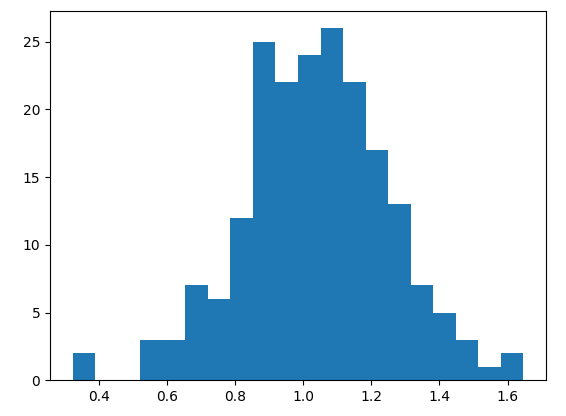
\includegraphics[scale=0.35]{Images/histo_linear_opti_rounded}
  \caption{Histogram of the merit factor values on a sequence of length 101 using the rounding scheme.}
  \label{fig:histo_linear_opti_rounded}
  \end{center}
\end{minipage}%
\hfill
\begin{minipage}{.45\textwidth}
  \begin{center}
  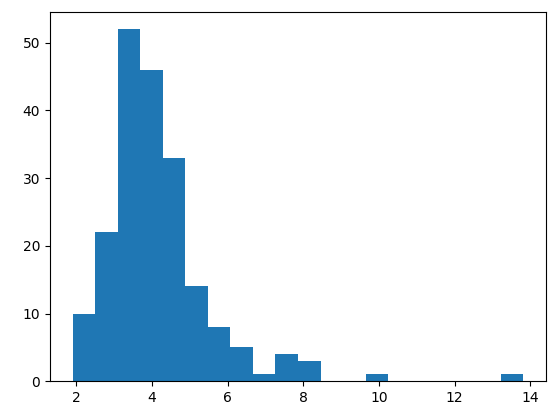
\includegraphics[scale=0.35]{Images/histo_linear_opti}
  \caption{Histogram of the merit factor values on a sequence of length 101 without rounding (with values between -1 and 1)}
  \label{fig:histo_linear_opti}
  \end{center}
\end{minipage}
\end{figure}
\noindent
The optimal result in this case is 8.82. Unfortunately, our rounding method (fig \ref{fig:histo_linear_opti_rounded}) has poor results and find solutions with a merit factor between 0 and 1.6. The not rounded solutions (fig \ref{fig:histo_linear_opti}) find results way better than the optimal integer one (around 14) which is legit because it solves a relaxed problem.\\
\textbf{Although this method is incredibly fast (0.15s in average for sequences of length 101), it yields very poor results.}

\begin{thebibliography}{999}

\bibitem{rls}Frank Neumanna, Ingo Wegener,\emph{Randomized local search, evolutionary algorithms, and the minimum spanning tree problem}.  
\bibitem{ea}Felix Streichert,\emph{Introduction to Evolutionary Algorithms}. 
\bibitem{sa}Scott Kirkpatrick, C. D. Gelatt, Mario P. Vecchi,\emph{Optimization by simulated annealing}.
\bibitem{mc}Cameron Browne, Edward Powley, Daniel Whitehouse,\emph{ A Survey of Monte Carlo Tree Search Methods}.  
\bibitem{max_quantum}Christoph Durr, Peter Høyer,\emph{A quantum algorithm for finding the minimum}.   
\bibitem{search}LK Grover,\emph{A fast quantum mechanical algorithm for database search}. 
\end{thebibliography}

\end{document}